\documentclass[conference]{IEEEtran}
\usepackage{blindtext, graphicx, algpseudocode, float, color}


% correct bad hyphenation here
\hyphenation{op-tical net-works semi-conduc-tor com-plexi-ty}


\begin{document}

\title{An Improvement of Controlling Quality of \\Large Scale Water-Level Data in Thailand}

\author{\IEEEauthorblockN{Nuttapon Pattanavijit}
\IEEEauthorblockA{
Department of Computer Engineering\\
Faculty of Engineering\\
Chulalongkorn University\\
Phayathai Road, Pathumwan\\
Bangkok, Thailand 10330\\
Email: nuttapon.p@student.chula.ac.th
}
\and
\IEEEauthorblockN{Peerapon Vateekul}
\IEEEauthorblockA{
Department of Computer Engineering\\
Faculty of Engineering\\
Chulalongkorn University\\
Phayathai Road, Pathumwan\\
Bangkok, Thailand 10330\\
Email: peerapon.v@chula.ac.th
}
\and
\IEEEauthorblockN{Kanoksri Sarinnapakorn}
\IEEEauthorblockA{
Hydro and Agro Informatics Institute\\
Ministry of Science and Technology\\
Thailand, 10400\\
Email: kanoksri@haii.or.th
}}

% make the title area
\maketitle


\begin{abstract}
%\boldmath
Extremely change in precipitation level such as water level can cause severe damage. In order to acknowledge changes, Hydro and Agro Informatics Institute has installed telemetry system across Thailand to collect and analyze precipitation level. However, to use its data in researching, incorrect data must be filtered. In previous work, we successfully detect various problems in water level data accurately. Still, missing pattern algorithm and outliers algorithm proposed in the previous work have run-time complexity up to $O(n^2)$, which are not quite suitable for large-scale data. In this paper, we aim to improve these algorithms, mainly focus on run-time complexity. As a result, we can speed up the outlier algorithm to $O(n)$ and the missing pattern to $O(n \log{n})$. Moreover, compared with the previous work, we measure actual running time of our algorithms and found that they significantly help reduce the running time.

\end{abstract}
% IEEEtran.cls defaults to using nonbold math in the Abstract.
% This preserves the distinction between vectors and scalars. However,
% if the journal you are submitting to favors bold math in the abstract,
% then you can use LaTeX's standard command \boldmath at the very start
% of the abstract to achieve this. Many IEEE journals frown on math
% in the abstract anyway.

% Note that keywords are not normally used for peerreview papers.
\begin{IEEEkeywords}
Purus, Vehicula, Ullamcorper, Dolor, Sollicitudin
\end{IEEEkeywords}

\IEEEpeerreviewmaketitle

\section{Introduction}

Thailand has faced many dreadful climate-related disaster including floods, droughts, and tropical cyclones. They have happened year after year and cause severe loss. For example, In 2011, seasonal flooding results in US\$ 45.7 billion damage to Thailand’s economy, which is 1.1\% of the country’s GDP [1]. Also, the climate-related disaster bring difficulties to agriculture and industry, which are backbones of Thailand economy.

To handle these disaster, the government established many organization to cooperatively counteract with it. One of the organization is Hydro and Agro Informatics Institute (HAII). HAII’s main focus is to research and utilize knowledge in agricultural and water resource management to confront the climate disaster [2].

In order to conduct researches, they have collected precipitation data by installing telemetry systems across Thailand. The telemetry system is a device that is used to collect physical, chemical, and biological data from its various sensors [3]. For instance, river’s water level, rainfall level, humidity, and temperature can be measured. Today, HAII have already installed over 800 telemetry systems. The data collected from the telemetry systems is sent back to HAII’s server by using GPRS cellular network [4].

Sometimes, incorrect data is reported from the telemetry systems such as minus value of cumulative rainfall level, or river’s water level suddenly changed from one level to another, which are not possible. In addition, data loss can also be occurred due to poor cellular network in rural area. These inconsistent data is not suitable to be used in researches since it might lead to inaccurate results.

To filtered out incorrect data efficiently, our previous work called “Controlling Quality of Water-Level Data in Thailand” proposed algorithms to detect anomalies in water level data, which includes outliers, inhomogeneity, and missing pattern algorithm [5]. Example of anomaly data detected by these algorithms is illustrated in figure \ref{fig:example_outliers}, figure \ref{fig:example_inhomogeneity}, and figure \ref{fig:example_missingpattern}. However, when we implement this algorithm to use with real precipitation level data, a problem arise. Since HAII use `R` as a main programming languages for all data analytic tasks, implementing outliers and missing pattern algorithm may leads to $O(n^2)$ in complexity. This inefficiency is originated from two main points. First, The bottleneck of both algorithms is occurred from clustering algorithm. The previous work use \textit{DBSCAN} [6] as the clustering algorithm which have $O(n^2)$ complexity if it is a naive implementation and $O(n\log{n})$ if it is implemented using special data structures that support fast region query such as \textit{R*-Tree} or \textit{k-d Tree} , which seem to be much more complex. Second, Our last work is implemented in HAII using \texttt{R} library called \texttt{fpc} which contains \textit{DBSCAN} library that have $O(n^2)$ complexity [7]. Thus, the overall algorithms’ complexity become $O(n^2)$.

\begin{figure}
	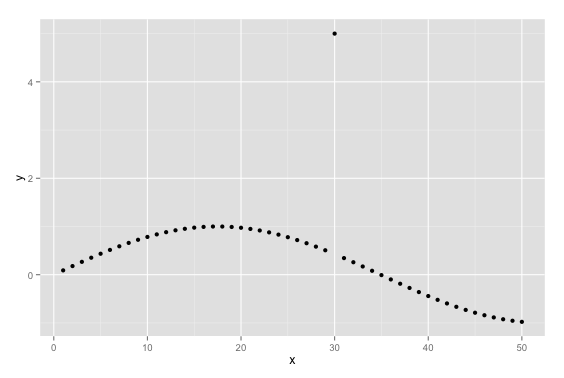
\includegraphics[width=\linewidth]{figure1.png}
	\caption{Example of data with outliers.}
	\label{fig:example_outliers}
\end{figure}

\begin{figure}
	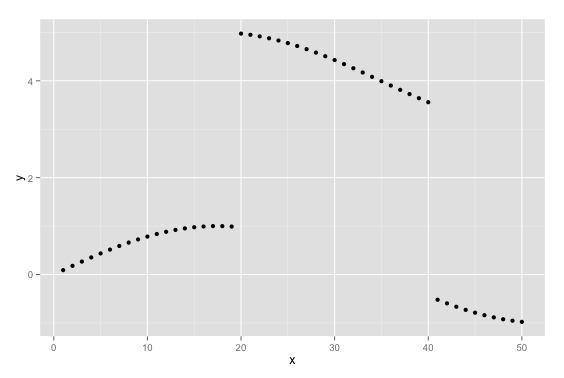
\includegraphics[width=\linewidth]{figure2.png}
	\caption{Example of data with inhomogeneity.}
	\label{fig:example_inhomogeneity}
\end{figure}

\begin{figure}
	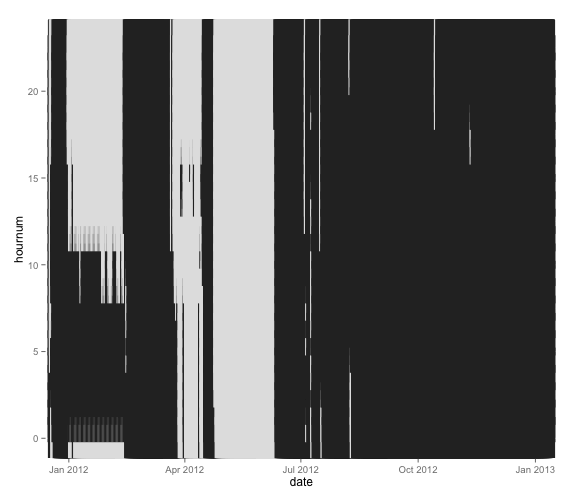
\includegraphics[width=\linewidth]{figure3.png}
	\caption{Example of data with missing pattern. X-axis represent date of the data. Y-axis indicate hour of day of the data. The lighter area shows date and hour where data was missing.}
	\label{fig:example_missingpattern}
\end{figure}

This paper aim to propose an improvement in outliers and missing pattern algorithms for large-scale water level data. Our main goal is to refine both algorithm to be simple, yet expeditious, while bring out the same results as our previous work. We have reduce running time of outliers algorithm from $O(n^2)$ or $O(n \log{n})$, depends on data structures, to $O(n)$. Also, missing pattern is decresed from $O(n^2)$ or $O(n \log^2{n})$ to $O(n \log{n})$. This can be  done by imitating the clustering result with more simple and fast approach which we will discuss later. The experimental result revealed that our approach significantly cuts down the overall running time in large-scale data.

The paper is organized as follows. Section 2 describes how data was collected at HAII. Section 3 recaps our previous work and points out problems. Our approach to refine the both algorithms are illustrated in Section 4. Experiment results are shown in Section 5. Last, Section 6 delivers a conclusion.

\section{Large-Scale Water Level Data}

Currently, Hydro and Agro Informatics Institute (HAII) have already installed over 800 telemetry system across Thailand. \textbf{\color{red}Add Map Figure!}Figure 4 shows example of location where telemetry systems were installed. Each system send data from its many sensors back to central database every 10 minutes via cellular network. From these numbers, we can estimate that there are 3.45 million records of data added to database every month. Since HAII have collected precipitation data for over 5 years, we can assume that we are dealing with approximately 207 million records. In previous paper, we use water level data for both outliers and missing pattern algorithms. Moreover, because of the nature of water level in the river, water level's value should be continuous without sudden change. Moreover, data is stored in timestamp order.

\section{Previous Data Quality Management}

Our previous work proposed two algorithms to control quality of water-level data, outliers and missing pattern. Both of the algorithms apply clustering technique in order to detect anomaly data and pattern of data. DBSCAN was selected as a clustering algorithms. Note that for the time dimension, 10 minutes will be counted as a distance of 1 unit because data points is captured in 10 minutes interval.

\subsection{Outliers Detection Algorithm}
In previous work, we detect outliers by directly applies \textit{DBSCAN} to water-level data. \textit{DBSCAN}'s required parameters, minimum number of points \textit{minpts} and distance epsilon \textit{eps}, is set to 3 and 1.05 respectively in order to classify data which have extreme difference in value compared to adjacent data as a noise. Figure \ref{fig:outliers_pseudocode} illustrates pseudocode of outliers detection algorithm.

\begin{figure}[H]
\begin{algorithmic}[1]
\Procedure{Detect-Outliers}{$d$}
\State $minpts\gets3$
\State $eps\gets1.05 $
\State $C\gets\emptyset$\Comment{Set of cluster of data index}
\State $N\gets\emptyset$\Comment{Set of noise data index}
\State $C, N \gets $\Call{DBSCAN}{$d, minpts, eps$}
\State \Return{$N$}
\EndProcedure
\end{algorithmic}
\caption{Pseudocode of outliers detection algorithm.}
\label{fig:outliers_pseudocode}
\end{figure}

From pseudocode in Figure \ref{fig:outliers_pseudocode}, it is obvious that running time of \textsc{Detect-Outliers} is based on \textsc{DBSCAN}. Thus, we can conclude that \textsc{Detect-Outliers} complexity is $O(n^2)$ or $O(n\log{n})$ -- depends on the data structure inside \textsc{DBSCAN}.

\subsection{Missing Pattern Algorithm}

Proposed in previous work, missing pattern is used to detect pattern of missing data. \textbf{\color{red}Add some conjunction sentencs here!} First, it convert water-level data into frequency domain, which count how many data is missing during each hour ($f_{0} ,f_{1}, \ldots, f_{23}$). Second, we use DBSCAN to analyze the frequency. If there are more than one cluster detected, there must be at least two hours having significantly different missing frequency $(f_{i})$. Then, we ... . Next, divided-and-conquer technique was applied to find missing pattern in subset of data. Last, we merge overlapped missing result together.

To be easier to explain, we rewrite its pseudocode from previous work in figure \ref{fig:missingpattern_pseudocode}. Result of \textsc{Missing-Pattern} procedure is returned as a list of tuples indicating start date and end date of pattern. Also, list is always sorted by start date of tuples.

\begin{figure}[H]
\begin{algorithmic}[1]
\Procedure{Missing-Pattern}{$d$}
\If{$end - start \le \textit{minDataReq}$}
\State\Return{$\emptyset$}\Comment{Too few data}
\EndIf
\State $f \gets$ \Call{Hourly-Missing-Frequency}{$d$}
\State $minpts \gets 1$
\State $eps \gets \frac{|d|}{2}$
\State $C, N \gets$ \Call{DBSCAN}{$f, minpts, eps$}
\State
\State $\textit{haveOverallMP} \gets |C| \ge 2$
\State
\State $P_{l} \gets$ \Call{Missing-Pattern}{$d_{1} \ldots d_{\frac{|d|}{2}}$}
\State $P_{r} \gets$ \Call{Missing-Pattern}{$d_{\frac{|d|}{2}+1} \ldots d_{|d|}$}
\State $P \gets$ \Call{Combine-Result}{$P_{l}, P_{r}, \textit{haveOverallPattern}$}
\State
\State $\textit{mergeGap} \gets 15$ \Comment{15 days}
\State \Return{\Call{Merge-Overlap-Pattern}{$P, \textit{mergeGap}$}}
\EndProcedure
\end{algorithmic}
\caption{Pseudocode of missing pattern algorithm.}
\label{fig:missingpattern_pseudocode}
\end{figure}

From figure \ref{fig:missingpattern_pseudocode}, \textsc{Hourly-Missing-Frequency} on line 5 can be done in $O(|d|)$ by using counting sort with 24 bucket representing missing frequency of each hour of day ($f_{0},\ldots,f_{23}$). \textsc{Combine-Result} on line 14 is done in $O(1)$ by checking 8 possible cases. And, \textsc{Merge-Overlap-Pattern} could be executed in $O(|d|)$. Since the tuples in $P$ is sorted and not literally overlap, we can sequentially check each adjacent pair of tuples whether it should be merged. We can conclude that \textsc{DBSCAN} is the bottleneck in each recursive call.

Since it uses divide-and-conquer, We can compute the complexity of by using \textit{master method}, which the complexity of algorithm can be represent in:

\[
T(n) = aT(\frac{n}{b}) + f(n)
\]

If \textsc{DBSCAN} have $O(n^2)$ complexity, the complexity of \textsc{Missing-Pattern} would be:

\[
T(n) = 2T(\frac{n}{2}) + O(n^2)
\]

By applying \textit{master theorem}, \textsc{Missing-Pattern}'s complexity become $O(n^2)$.

On the other hand, If \textsc{DBSCAN} have $O(n \log{n})$ complexity, the complexity of \textsc{Missing-Pattern} would be:
\[
T(n) = 2T(\frac{n}{2}) + O(n \log{n})
\]

By applying \textit{master theorem}, \textsc{Missing-Pattern}'s complexity become $O(n \log^2{n})$.


\section{Proposed Improved Algorithms}
Our proposed algorithms aim to solve the bottleneck in both algorithms in order to make them faster. To do that, we try to create a new clustering algorithm which can imitate \textit{DBSCAN}'s result but with more efficiency, by using some facts about precipitation data and the algorithms themselves.

%First, since the data was captured from a sensor, we can assume that at time $t$, there will be only one $d_{t}$. This fact implies that there is no need to search for adjacent point in two dimension. Also, the data is already sorted by time. So, searching for data points that have distance from $d_{t}$ less than $\epsilon$ can be done in linear time by looking forward and backward from $d_{t}$. In other words, we can try to increase $j$ then check the distance between $d_{t}$ and $d_{t+j}$ until the distance is greater than $\epsilon$. On the other hand, looking backward for distance between $d_{t}$ and $d_{t-i}$ can be done in the same way. We can say that finding $i_{max}$, $j_{max}$ for
%\[
%D = \{d_{t-i}, \ldots, d_{t}, \ldots, d_{t+j}\}
%\]
%
%where
%
%\[
%|d_{t-i} - d_{t}|\le\epsilon\textit{ and }|d_{t+j} - d_{t}|\le\epsilon
%\]
%can be done in linear time.

First, since the data was captured from a sensor, we can assume that at time $t$, there will be only one $d_{t}$. This fact implies that there is no need to search for adjacent points in two dimension.

Second, outliers algorithm and missing pattern algorithm produce best result when $\textit{minpts} = 3$ and $\textit{minpts} = 1$ respectively. Let $C_{k}$ be the set of cluster of data index. We can say that if $\textit{minpts} \le 3$, following properties are always true:
%\begin{enumerate}
%	\item if $d_{i}$ is in $C_{k}$ (\textit{$k^{th}$} cluster) and $|d_{i+1} - d_{i}| \le \textit{eps}$, then $d_{i+1}$ is in $C_{k}$ too.
%	\item $|C_{k}| \ge \textit{minpts}$ for all $k$ 
%\end{enumerate}
\begin{enumerate}
	\item if $i$ is in $C_{k}$ (\textit{$k^{th}$} cluster) and $|d_{i+1} - d_{i}| \le \textit{eps}$, then $i+1$ is in $C_{k}$ too.
	\item $|C_{k}| \ge \textit{minpts}$ for all $k$ 
\end{enumerate}

The first property is true because if $\textit{minpts} = 1$, at least $d_{i}$ can form its own cluster and add $d_{i+1}$ to its cluster. If $\textit{minpts} = 2$ and $i$ is in $C_{k}$, there must be another data point $j \in C_{k}, j < i$ within distance $\textit{eps}$. So $i$ can be add freely into $C_{k}$. Last, if $\textit{minpts} = 3$, since $i$ is already in $C_{k}$, there must be another data point $j \in C_{k}, j < i$ within distance $\textit{eps}$. So, if $|d_{i+1} - d_{i}| \le \textit{eps}$, $d_{i}$ will satisfy $\textit{minpts} = 3$ (including itself) condition and $i+1$ can be added into $C_{k}$.

For the second property, assume that $C_{k}$ is the smallest cluster possible, $C_{k}$ must have at least one core data point in order to form a cluster. Let $d_{k}$ be the only core data point. $d_{k}$ must have at least $\textit{minpts}$ data point within distance $\textit{eps}$ (including itself). So, we can conclude that $|C_{k}| \ge \textit{minpts}$.

With this two properties, we can create an algorithm which can imitate \textit{DBSCAN}'s result for $\textit{minpts} \le 3$. Figure \ref{fig:clustering_pseudocode} illustrates its pseudocode.

\begin{figure}[H]
\begin{algorithmic}[1]
\Procedure{Linear-Cluster}{$d, minpts, eps$}
\State $C \gets \emptyset$
\State $N \gets \emptyset$
\State $c \gets \{1\}$\Comment{Temporary Cluster}
\For{$i \gets 2,|d|$}
	\If{$|d_{i} - d_{i-1}| < eps$}
\State	$c \gets c \cup \{i\}$
	\Else
		\If{$|c| \ge minpts$}
\State		$C \gets C \cup \{c\}$
		\Else
\State		$N \gets N \cup c$
		\EndIf
		\State $c \gets \emptyset$
	\EndIf
\EndFor
\State
\If{$|c| \ge minpts$}
\State		$C \gets C \cup \{c\}$
\Else
\State		$N \gets N \cup c$
\EndIf
\State
\State	\Return{$C, N$}
\EndProcedure
\end{algorithmic}
\caption{Pseudocode of new clustering algorithm.}
\label{fig:clustering_pseudocode}
\end{figure}

From figure \ref{fig:clustering_pseudocode}, the pseudocode work by following steps. First, it creates a temporary cluster an assume that $d_{i}$ is in cluster (start from $d_{1}$). Then, it checks the distance to its next adjacent data point ($d_{i+1}$). If the distance is less than $eps$, put $d_{i+1}$ in the same temporary cluster. Otherwise, create new temporary cluster and assume that $d_{i+1}$ is in it. Before creating new temporary cluster, we determine whether the previous temporary cluster can be formed into real cluster or not by counting data points inside it. If it has more than $minpts$ points, it can be formed as a real cluster. If not, all data point inside it should be considered as noise. Thus, the algorithm obviously has $O(n)$ complexity since it contains only one for-loop from $2$ to $|d|$.

Therefore, we can replace \textit{DBSCAN} in outliers algorithm and missing pattern algorithm with \textsc{Linear-Cluster} to reduce it's overall complexity. The outliers algorithm is become $O(n)$ in complexity.


\section{Experiments}

Lorem Ipsum

\section{Conclusion}

Lorem Ipsum

\begin{thebibliography}{1}

\bibitem{IEEEhowto:kopka}
H.~Kopka and P.~W. Daly, \emph{A Guide to \LaTeX}, 3rd~ed.\hskip 1em plus
  0.5em minus 0.4em\relax Harlow, England: Addison-Wesley, 1999.

\end{thebibliography}

\end{document}


